\documentclass[12pt, a4paper]{report}

% =========================================================
% 1. PREAMBLE & PACKAGES
% =========================================================

% --- Mathematics & Symbols (MUST BE LOADED FIRST) ---
\usepackage{amsmath}    
\usepackage{amssymb}    % <--- Defines \mathbb{R}
\usepackage{amsfonts}   

% --- Language & Fonts ---
\usepackage[utf8]{inputenc}
\usepackage[T1]{fontenc}
\usepackage[utf8]{vietnam} % Loads AFTER math packages
\usepackage{helvet}        
\renewcommand{\familydefault}{\sfdefault} 
\usepackage[english]{babel}

% --- Page Layout & Graphics ---
\usepackage[a4paper, top=2.5cm, bottom=2.5cm, left=2cm, right=2cm, headheight=35pt]{geometry}
\usepackage{graphicx}
\usepackage{xcolor}
\usepackage{tikz}       
\usetikzlibrary{calc}

% --- HEADER AND FOOTER CONFIGURATION ---
\usepackage{fancyhdr}
\usepackage{lastpage} 

% Header
\newcommand{\myHeaderContent}{
    \lhead{
\includegraphics[height=0.6cm]{HCMUT_official_logo.png} \hspace{0.5cm}\bfseries University of Technology, Ho Chi Minh City} 
    \chead{}
    \rhead{\small Academic Year 2025 - 2026} 
}

% Footer
\newcommand{\myFooterContent}{
    \lfoot{\bfseries Linear Algebra}
    \cfoot{PCA: Data Dimensionality Reduction} 
    \rfoot{Page \thepage/\pageref{LastPage}}
}

\pagestyle{fancy}
\fancyhf{} 
\myHeaderContent
\myFooterContent
\renewcommand{\headrulewidth}{1pt} 
\renewcommand{\footrulewidth}{1pt} 

\fancypagestyle{plain}{%
  \fancyhf{}%
  \myHeaderContent
  \myFooterContent
  \renewcommand{\headrulewidth}{1pt} 
  \renewcommand{\footrulewidth}{1pt} 
}

% --- Tables & Formatting Tools ---
\usepackage{scrextend}
\usepackage{array, booktabs, multicol, multirow, siunitx, tabularx}
\setlength{\parindent}{0pt}
\setlength{\parskip}{6pt}

% --- Code Listings ---
\usepackage{listings}
\definecolor{codegreen}{rgb}{0,0.6,0}
\definecolor{codegray}{rgb}{0.5,0.5,0.5}
\definecolor{codepurple}{rgb}{0.58,0,0.82}
\definecolor{backcolour}{rgb}{0.95,0.95,0.92}

\lstdefinestyle{mystyle}{
    backgroundcolor=\color{backcolour},   
    commentstyle=\color{codegreen},
    keywordstyle=\color{magenta},
    numberstyle=\tiny\color{codegray},
    stringstyle=\color{codepurple},
    basicstyle=\ttfamily\footnotesize,
    breakatwhitespace=false,         
    breaklines=true,                 
    captionpos=b,                    
    keepspaces=true,                 
    numbers=none,                    
    numbersep=5pt,                  
    showspaces=false,                
    showstringspaces=false,
    showtabs=false,                  
    tabsize=2,
    extendedchars=true 
}
\lstset{style=mystyle}

% --- URL and Hyperlinks ---
\usepackage[hyphens]{url}                 
\usepackage[hidelinks]{hyperref} 

% --- Table of Contents Config ---
\usepackage{tocloft}

\AtBeginDocument{
    \renewcommand{\contentsname}{\hfill\bfseries\Large\underline{TABLE OF CONTENTS}\hfill}
}
\renewcommand{\cfttoctitlefont}{} 
\renewcommand{\cftaftertoctitle}{}
\renewcommand{\cftchappresnum}{\bfseries CHAPTER }
\renewcommand{\cftchapaftersnum}{: }
\setlength{\cftchapnumwidth}{8em}
\renewcommand{\cftchapleader}{\cftdotfill{\cftdotsep}}
\renewcommand{\cftchapfont}{\bfseries}
\renewcommand{\cftchappagefont}{\bfseries}
\setlength{\cftsecindent}{2em}    
\setlength{\cftsubsecindent}{4.5em}
\renewcommand{\cftsecfont}{\normalfont}
\renewcommand{\cftsecpagefont}{\normalfont}

% =========================================================
% 3. DOCUMENT CONTENT
% =========================================================
\begin{document}

% --- TITLE PAGE ---
\begin{titlepage}
    % The Blue Border Logic
    \begin{tikzpicture}[remember picture,overlay,inner sep=0,outer sep=0]
         \draw[blue!70!black,line width=4pt] ([xshift=-1.5cm,yshift=-2cm]current page.north east) coordinate (A)--([xshift=1.5cm,yshift=-2cm]current page.north west) coordinate(B)--([xshift=1.5cm,yshift=2cm]current page.south west) coordinate (C)--([xshift=-1.5cm,yshift=2cm]current page.south east) coordinate(D)--cycle;

         \draw ([yshift=0.5cm,xshift=-0.5cm]A)-- ([yshift=0.5cm,xshift=0.5cm]B)--
         ([yshift=-0.5cm,xshift=0.5cm]B) --([yshift=-0.5cm,xshift=-0.5cm]B)--([yshift=0.5cm,xshift=-0.5cm]C)--([yshift=0.5cm,xshift=0.5cm]C)--([yshift=-0.5cm,xshift=0.5cm]C)-- ([yshift=-0.5cm,xshift=-0.5cm]D)--([yshift=0.5cm,xshift=-0.5cm]D)--([yshift=0.5cm,xshift=0.5cm]D)--([yshift=-0.5cm,xshift=0.5cm]A)--([yshift=-0.5cm,xshift=-0.5cm]A)--([yshift=0.5cm,xshift=-0.5cm]A);

         \draw ([yshift=-0.3cm,xshift=0.3cm]A)-- ([yshift=-0.3cm,xshift=-0.3cm]B)--
         ([yshift=0.3cm,xshift=-0.3cm]B) --([yshift=0.3cm,xshift=0.3cm]B)--([yshift=-0.3cm,xshift=0.3cm]C)--([yshift=-0.3cm,xshift=-0.3cm]C)--([yshift=0.3cm,xshift=-0.3cm]C)-- ([yshift=0.3cm,xshift=0.3cm]D)--([yshift=-0.3cm,xshift=0.3cm]D)--([yshift=-0.3cm,xshift=-0.3cm]D)--([yshift=0.3cm,xshift=-0.3cm]A)--([yshift=0.3cm,xshift=0.3cm]A)--([yshift=-0.3cm,xshift=0.3cm]A);
    \end{tikzpicture}

    \begin{center}
        \vspace{7pt}
        \textbf{
        VIETNAM NATIONAL UNIVERSITY\\
        HO CHI MINH CITY UNIVERSITY OF TECHNOLOGY \\
        }
        \vspace{7pt}
        \textbf{FACULTY OF APPLIED SCIENCE}
    \end{center}

    \vspace{5pt}
    \begin{center}
        % LOGO PLACEHOLDER FOR TITLE PAGE
        
\includegraphics[scale=0.7]{HCMUT_official_logo.png}
    \end{center}

    \vspace{5pt}
    \begin{center}
        \begin{tabular}{c}
          \textbf{\Huge LINEAR ALGEBRA}         \\
          \\
           \textbf{\ Sem 251  - CC02 - Group 02}          \\
          {}                                             \\
          \midrule                    
          \\
         \textbf{\normalsize
        \parbox{13cm}{\centering PRINCIPAL COMPONENT ANALYSIS: DATA DIMENSIONALITY REDUCTION}
        }
        \\
          {}                                           \\
          \bottomrule
        \end{tabular}
    \end{center}

    \vspace{0.1cm}
    \begin{center}
        \textbf{\ Instructor: Phan Thi Khanh Van}   
    \end{center}

    \begin{table}[h]
        \begin{tabular}{rll}
            \hspace{3cm}Students: & Dao Tan Vy (Leader) & ID 2551458 \\
                                  & Nguyen Hoang Vinh Phuc & ID 2551446 \\
                                  & Nguyen Chi Duc & ID 2551425 \\
                                  & Nguyen Hoang Dang Khoa & ID 2452546 \\
                                  & Nguyen Nam Son & ID 2353051 \\
        \end{tabular}
    \end{table}

    \vspace{0cm}
    \begin{center}
        \textbf{Ho Chi Minh, 2025}
    \end{center}
\end{titlepage}

% --- TABLE OF CONTENTS ---
\pagenumbering{roman} % Start Roman numerals (i, ii) for ToC
\tableofcontents

% --- CHAPTER CONTENT ---

% --- INTRODUCTION ---
\newpage
\pagenumbering{arabic} % Switch to Arabic numbers (1, 2)
\setcounter{page}{1}   % Start counting from 1
\phantomsection
\addcontentsline{toc}{chapter}{\MakeUppercase{Introduction}} 
\chapter*{\MakeUppercase{Introduction}} 

Principal Component Analysis (PCA) is a dimensionality-reduction technique that transforms high-dimensional data into a smaller set of new variables called principal components, which capture the most important patterns in the data.

By focusing on directions of maximum variance, PCA helps simplify complex datasets, reduce noise, and improve visualization or model performance while preserving as much essential information as possible. It is widely used in fields such as machine learning, finance, image processing, and biology.

The objectives of this project include:
\begin{itemize}
    \item Understanding the theoretical foundations of PCA.
    \item Applying matrix operations to solve real-world problems.
    \item Using MATLAB to simulate and calculate results efficiently.
\end{itemize}

% CHAPTER 1
\newpage
\chapter{\MakeUppercase{Overview}}

\section{Problem Definition: Data Dimensionality}

\subsection{Definition of Data Dimensionality}
Data dimensionality refers to the number of features (variables or attributes) present in a dataset. For a dataset with $n$ samples and $p$ features, the dimensionality is defined as $p$.

\subsection{The Curse of Dimensionality}
High-dimensional data presents several challenges, often referred to as the "Curse of Dimensionality". These challenges include:
\begin{itemize}
    \item \textbf{Exponential increase in volume:} As dimensions increase, the data becomes sparse.
    \item \textbf{Distance metrics:} Distances between data points become less meaningful in high-dimensional space.
    \item \textbf{Computational cost:} High dimensionality leads to increased computational cost and memory usage.
    \item \textbf{Overfitting:} There is a higher risk of overfitting in machine learning models.
    \item \textbf{Visualization:} It is difficult for humans to visualize data beyond 3 dimensions.
\end{itemize}

\subsection{Why Dimensionality Reduction is Needed}
Dimensionality reduction is crucial to remove redundant or noisy features and retain the most important information. It helps to speed up algorithms, improve model generalization, and enable better visualization of complex datasets.

\subsection{Types of Dimensionality Reduction Techniques}
Techniques are generally categorized into:
\begin{itemize}
    \item \textbf{Linear methods:} Such as Principal Component Analysis (PCA) and Linear Discriminant Analysis (LDA).
    \item \textbf{Non-linear methods:} Such as t-SNE, UMAP, and Autoencoders.
    \item \textbf{Justification for choosing PCA:} 
For this study, we selected PCA over non-linear methods like t-SNE because \textbf{interpretability} is our priority. While t-SNE is excellent for clustering, it distorts the feature space, making it impossible to tell which original variables (e.g., "Deaths" vs "Damage") caused the separation. PCA preserves the linear weights (loadings), allowing us to construct a Biplot that explicitly links disaster severity to specific economic or human costs.
\end{itemize}

\section{Introduction to PCA}

\subsection{What is Principal Component Analysis?}
Principal Component Analysis (PCA) is a linear transformation technique that projects high-dimensional data onto a new coordinate system known as principal components. In this new system:
\begin{itemize}
    \item The \textbf{first principal component} captures the direction of maximum variance.
    \item Each \textbf{subsequent component} captures the maximum remaining variance while being orthogonal to the previous ones.
\end{itemize}

\subsection{Historical Background}
PCA was invented by Karl Pearson in 1901 and later developed by Harold Hotelling in 1933 as a statistical tool.

\subsection{Key Intuition}
The key intuition behind PCA is to find the "best" lower-dimensional subspace that preserves as much variability (information) as possible from the original dataset.

\subsection{Illustrative Example}
Consider a 2D dataset, such as the height versus weight of people. PCA rotates the axes to align with the direction of the greatest spread (variance) of the data.

\begin{figure}[h]
    \centering
    \begin{tikzpicture}[scale=1.0]
        % 1. Draw Grid (Optional, for reference)
        \draw[step=1cm,gray!10,very thin] (-1,-1) grid (6,6);

        % 2. Draw Original Axes (x and y)
        \draw[->, thick, black!70] (0,0) -- (5.5,0) node[right] {\small Original $x$ (e.g. Height)};
        \draw[->, thick, black!70] (0,0) -- (0,5.5) node[above] {\small Original $y$ (e.g. Weight)};

        % 3. Draw Data Points (Simulated cloud with positive correlation)
        % These points form a diagonal elliptical shape
        \foreach \p in {
            (1.0,1.2), (1.2,0.8), (1.5,1.6), (1.8,1.5), 
            (2.0,2.1), (2.2,1.9), (2.5,2.8), (2.8,2.4), 
            (3.0,3.3), (3.2,2.9), (3.5,3.6), (3.8,3.4), 
            (4.0,4.2), (4.2,3.8), (2.6, 2.6), (2.4, 2.2)
        }{
            \fill[blue!60] \p circle (2.5pt);
        }

        % 4. Draw Principal Component Axes (Rotated)
        % We center these at the "mean" of our data (approx 2.7, 2.7)
        \coordinate (Mean) at (2.7, 2.7);

        % PC1: Direction of Maximum Variance (The long axis)
        \draw[->, red, very thick] (Mean) -- ++(2.2, 2.2) node[right] {\textbf{PC1} (Max Variance)};
        \draw[-, red, dashed] (Mean) -- ++(-1.5, -1.5); % Backward extension line

        % PC2: Orthogonal Direction (The short axis)
        \draw[->, orange, very thick] (Mean) -- ++(-1.2, 1.2) node[left] {\textbf{PC2}};
        
        % 5. Add an angle arc to show rotation
        \draw[->, black, thin] (1,0) arc (0:45:1) node[midway, right] {\scriptsize $\theta$};

    \end{tikzpicture}
    \caption{Visualizing PCA: The red axes ($PC_1, PC_2$) are rotated to align with the data's greatest spread, distinct from the original $x, y$ axes.}
    \label{fig:pca_visual}
\end{figure}

\subsection{Relationship with Other Methods}
PCA is closely related to Singular Value Decomposition (SVD) and can be viewed as a special case of factor analysis.

\section{Objectives, Advantages, and Disadvantages}

\subsection{Main Objectives}
The primary goals of applying PCA are:
\begin{itemize}
    \item Maximize preserved variance while minimizing the number of dimensions.
    \item Decorrelate features (principal components are orthogonal and uncorrelated).
    \item Enable visualization of high-dimensional data (e.g., reducing to 2D or 3D).
    \item Improve performance and reduce overfitting in downstream machine learning tasks.
    \item Reduce noise by discarding low-variance components.
\end{itemize}

\subsection{Advantages}
PCA offers several significant benefits:
\begin{itemize}
    \item \textbf{Efficiency:} It is computationally efficient and scalable, especially with SVD-based implementations.
    \item \textbf{Unsupervised:} It does not require labeled data.
    \item \textbf{Deterministic:} The same input always yields the same result.
    \item \textbf{Accessibility:} It is widely available in libraries such as scikit-learn, MATLAB, and R.
    \item \textbf{Foundation:} It has a strong mathematical foundation and interpretability regarding variance.
\end{itemize}

\subsection{Disadvantages}
Despite its utility, PCA has limitations:
\begin{itemize}
    \item \textbf{Linearity Assumption:} PCA assumes linear relationships and fails to capture non-linear structures (manifold learning or Kernel PCA may be required).
    \item \textbf{Interpretability:} Principal components are linear combinations of original features, which can be semantically hard to interpret.
    \item \textbf{Scaling Sensitivity:} Features must be standardized beforehand as PCA is sensitive to the scale of data.
    \item \textbf{Outliers:} PCA is sensitive to outliers, which can dominate the variance.
    \item \textbf{Information Definition:} It assumes variance is the best measure of information, which is not always true for classification tasks.
\end{itemize}





% =========================================================
% CHAPTER 2: MATHEMATICAL FOUNDATIONS
% =========================================================
\newpage
\chapter{Mathematical Foundations}

This chapter establishes the statistical and algebraic framework necessary for understanding Principal Component Analysis (PCA), including expectation, covariance, and eigen-decomposition.

% ---------------------------------------------------------
% 2.1 STATISTICAL FEATURES
% ---------------------------------------------------------
\section{Statistical Features}

\subsection{Expectation}
The expectation of a random variable $X$, denoted $E[X]$, is the theoretical long-run average value of $X$. It represents the center or "balance point" of the distribution.

\textbf{For a Discrete Random Variable:}
If $X$ takes values $x_1, x_2, \dots, x_n$ with probabilities $p_1, p_2, \dots, p_n$:
\begin{equation}
    E[X] = \sum_{i=1}^{n} x_i p_i
\end{equation}

\textbf{For a Continuous Random Variable:}
If $X$ has a probability density function $f(x)$:
\begin{equation}
    E[X] = \int_{-\infty}^{\infty} x f(x) \, dx
\end{equation}

\subsection{Variance}
Variance measures how spread out the values of a random variable are around the mean. A higher variance means the data is more dispersed.

\textbf{Formula:}
\begin{equation}
    \text{Var}(X) = E[(X - E[X])^2]
\end{equation}
This is the expected (average) squared distance from the mean.

\textbf{Equivalent Computational Formula:}
\begin{equation}
    \text{Var}(X) = E[X^2] - (E[X])^2
\end{equation}

\subsection{Standard Deviation}
Standard deviation is the square root of variance:
\begin{equation}
    \sigma = \sqrt{\text{Var}(X)}
\end{equation}

% ---------------------------------------------------------
% 2.2 COVARIANCE
% ---------------------------------------------------------
\section{Covariance}

\subsection{Definition (Scalar)}
For integrable random variables $X$ and $Y$:
\begin{equation}
    \text{Cov}(X,Y) := E[(X - E[X])(Y - E[Y])] = E[XY] - E[X]E[Y]
\end{equation}
Note that the variance of $X$ is simply the covariance of $X$ with itself:
\[ \text{Var}(X) = \text{Cov}(X, X) \]

\subsection{Properties}
\begin{itemize}
    \item \textbf{Symmetry:} $\text{Cov}(X, Y) = \text{Cov}(Y, X)$.
    \item \textbf{Bilinearity:} Covariance is bilinear in both arguments:
    \[ \text{Cov}(aX + bY, Z) = a\text{Cov}(X, Z) + b\text{Cov}(Y, Z) \]
    \item \textbf{Relation to Independence:} If $X$ and $Y$ are independent (and integrable), then $\text{Cov}(X, Y) = 0$.
    \begin{itemize}
        \item \textit{Note:} The converse is false; covariance zero does \textbf{not} imply independence in general.
    \end{itemize}
    \item \textbf{Cauchy–Schwarz Bound:}
    \[ |\text{Cov}(X, Y)| \leq \sqrt{\text{Var}(X)\text{Var}(Y)} \]
    This yields the \textbf{correlation coefficient} $\rho_{X,Y}$:
    \[ \rho_{X,Y} = \frac{\text{Cov}(X, Y)}{\sqrt{\text{Var}(X)\text{Var}(Y)}}, \quad |\rho| \leq 1 \]
\end{itemize}

\subsection{Covariance Matrix (Multivariate)}
Let $X = (X_1, \dots, X_n)^\top$ be a random vector with finite second moments. Define the \textbf{covariance matrix} $\Sigma$:
\begin{equation}
    \Sigma := \text{Cov}(X) = E[(X - \mu)(X - \mu)^\top], \quad \text{where } \mu = E[X]
\end{equation}
The entries are given by $\Sigma_{ij} = \text{Cov}(X_i, X_j)$.

\textbf{Key Facts:}
\begin{itemize}
    \item $\Sigma$ is symmetric: $\Sigma^\top = \Sigma$.
    \item $\Sigma$ is positive semidefinite (PSD): For any vector $a \in \mathbb{R}^n$:
    \[ a^\top \Sigma a = \text{Var}(a^\top X) \geq 0 \]
    \item If all components have finite variance, then $\Sigma$ is finite.
\end{itemize}

\subsection{Conditional Covariance and Law of Total Covariance}
\begin{itemize}
    \item \textbf{Law of Total Expectation:} $E[X] = E[E[X|Y]]$.
    \item \textbf{Law of Total Covariance:}
    \begin{equation}
        \text{Cov}(X, Z) = E[\text{Cov}(X, Z|Y)] + \text{Cov}(E[X|Y], E[Z|Y])
    \end{equation}
    \item \textbf{Law of Total Variance} (Special case):
    \[ \text{Var}(X) = E[\text{Var}(X|Y)] + \text{Var}(E[X|Y]) \]
\end{itemize}

\subsection{Whitening / Decorrelation}
Given a positive definite covariance matrix $\Sigma$, one can compute a \textbf{whitening matrix} $W$ such that:
\[ W \Sigma W^\top = I \]
Common choices for $W$:
\begin{itemize}
    \item $W = \Sigma^{-1/2}$ (via eigen-decomposition).
    \item $W = L^{-1}$ (via Cholesky decomposition $\Sigma = LL^\top$).
\end{itemize}
Whitening removes covariances (resulting in an identity covariance matrix) and is often used as preprocessing for algorithms like ICA.

\subsection{Difference Between Diagonal and Off-Diagonal Values}
A covariance matrix summarizes how pairs of features vary together. For features $X_1, \dots, X_n$:
\[
\Sigma = \begin{pmatrix}
\text{Cov}(X_1, X_1) & \cdots & \text{Cov}(X_1, X_n) \\
\vdots & \ddots & \vdots \\
\text{Cov}(X_n, X_1) & \cdots & \text{Cov}(X_n, X_n)
\end{pmatrix}
\]

\textbf{1. Diagonal Values (Variances):}
Entries $\text{Cov}(X_i, X_i) = \text{Var}(X_i)$ describe the spread of a single dimension.
\begin{itemize}
    \item \textbf{Large variance:} The feature values vary significantly.
    \item \textbf{Small variance:} The feature values are tightly clustered around the mean.
\end{itemize}

\textbf{2. Off-Diagonal Values (Covariances):}
Entries $\text{Cov}(X_i, X_j)$ where $i \neq j$ describe how two features vary together.
\begin{itemize}
    \item \textbf{Positive:} When $X_i$ increases, $X_j$ tends to increase.
    \item \textbf{Negative:} When $X_i$ increases, $X_j$ tends to decrease.
    \item \textbf{Zero:} Features are uncorrelated.
\end{itemize}
These values reflect the shape and orientation of the data cloud in multivariate space.

% ---------------------------------------------------------
% 2.3 EIGENVALUES & EIGENVECTORS
% ---------------------------------------------------------
\section{Eigenvalues and Eigenvectors}

\subsection{Algebraic Definition}
For a square $n \times n$ matrix $A$, a scalar $\lambda$ is an \textbf{eigenvalue} and a non-zero vector $v$ is an \textbf{eigenvector} if:
\begin{equation}
    Av = \lambda v
\end{equation}
Equivalently, $\lambda$ is a root of the characteristic polynomial:
\[ p_A(\lambda) := \det(A - \lambda I) = 0 \]

\textbf{Multiplicity:}
\begin{itemize}
    \item \textbf{Algebraic multiplicity:} Multiplicity of $\lambda$ as a root of $p_A(\lambda)$.
    \item \textbf{Geometric multiplicity:} Dimension of the nullspace $\ker(A - \lambda I)$ (number of linearly independent eigenvectors).
    \item Always $1 \leq \text{geom mult} \leq \text{alg mult}$.
\end{itemize}

\subsection{Spectral Properties}
\begin{itemize}
    \item \textbf{Trace:} $\text{tr}(A) = \sum \lambda_i$ (sum of eigenvalues).
    \item \textbf{Determinant:} $\det(A) = \prod \lambda_i$ (product of eigenvalues).
    \item \textbf{Real Symmetric Matrices:} All eigenvalues are real, and eigenvectors can be chosen to be orthonormal (Spectral Theorem).
\end{itemize}

\subsection{Singular Value Decomposition (SVD)}
For any $m \times n$ real matrix $M$, SVD writes:
\begin{equation}
    M = U \Sigma V^\top
\end{equation}
Where $U$ and $V$ are orthogonal matrices, and $\Sigma$ is a diagonal matrix with non-negative \textbf{singular values} $\sigma_1 \geq \sigma_2 \geq \dots \geq 0$.
\begin{itemize}
    \item The singular values of $M$ are the square roots of the eigenvalues of $M^\top M$ (or $MM^\top$).
    \item SVD generalizes eigen-decomposition to non-square matrices and is numerically stable.
\end{itemize}

\subsection{Eigen-decomposition of Covariance Matrices \& PCA}
The covariance matrix $\Sigma$ is symmetric and positive semidefinite. Its eigen-decomposition is:
\begin{equation}
    \Sigma = Q \Lambda Q^\top
\end{equation}
where $Q$ is orthonormal and $\Lambda = \text{diag}(\lambda_1 \geq \lambda_2 \geq \dots \geq 0)$.

\textbf{Relation to PCA:}
\begin{itemize}
    \item \textbf{Principal Components:} The eigenvectors corresponding to the largest eigenvalues.
    \item \textbf{Variance Explained:} The variance explained by the $k$-th principal component is equal to $\lambda_k$.
    \item PCA projects mean-centered data onto the first $r$ eigenvectors to create a lower-dimensional representation that preserves maximal variance.
\end{itemize}

% =========================================================
% CHAPTER 3: THE PCA ALGORITHM
% =========================================================
\newpage
\chapter{The Principal Component Analysis Algorithm}

\section{Theoretical Framework}
Principal Component Analysis (PCA) is a dimensionality reduction technique that transforms a high-dimensional dataset into a smaller set of uncorrelated variables called Principal Components, while retaining as much of the original variation as possible [1]. The algorithm follows a rigorous five-step process.

\subsection{Step 1: Standardization (Data Scaling)}
The first step is to standardize the range of the continuous initial variables so that each of them contributes equally to the analysis. If there are large differences between the ranges of initial variables, those variables with larger ranges will dominate over those with small ranges.

For example, a "Damage Cost" variable ranging in the millions will mathematically overpower a "Death Count" variable ranging in the tens [2]. Transforming the data to comparable scales prevents this problem. We typically do this using the Z-score normalization:
\begin{equation}
    z = \frac{x - \mu}{\sigma}
\end{equation}
Where $x$ is the original value, $\mu$ is the mean, and $\sigma$ is the standard deviation. This results in a dataset where every variable has a mean of 0 and a variance of 1 [2].

\subsection{Step 2: Covariance Matrix Computation}
The aim of this step is to understand how the variables of the input data set are varying from the mean with respect to each other. The covariance matrix ($\Sigma$) is a symmetric matrix that has as entries the covariances associated with all possible pairs of the initial variables [3].

\begin{equation}
    \Sigma = \frac{1}{n-1} X^T X
\end{equation}

Since the covariance of a variable with itself is its variance, the main diagonal contains the variances of each initial variable. High positive values indicate variables that increase together, while zero values indicate no relationship.

\subsection{Step 3: Compute the Eigenvectors and Eigenvalues}
Eigenvectors and eigenvalues are the linear algebra concepts that we need to compute from the covariance matrix in order to determine the principal components of the data [3].
\begin{itemize}
    \item \textbf{Eigenvectors ($v$):} Determine the directions of the new feature space (where the data is most spread out).
    \item \textbf{Eigenvalues ($\lambda$):} Determine the magnitude (or variance) of the data along those new directions.
\end{itemize}
Mathematically, we solve the characteristic equation:
\begin{equation}
    \det(\Sigma - \lambda I) = 0
\end{equation}

\subsection{Step 4: Feature Vector Selection}
Once eigenvectors are found, we order them by their eigenvalues, from highest to lowest ($\lambda_1 \geq \lambda_2 \dots$). This gives us the components in order of significance. The eigenvector with the highest eigenvalue is the First Principal Component (PC1) [1].

We then choose to keep the top $k$ eigenvectors to form our feature vector $W$. This is the step where dimensionality reduction actually occurs, as we discard the components with low information (noise).

\subsection{Step 5: Projection (Recasting the Data)}
In the final step, we use the feature vector $W$ formed in the previous step to reorient the data from the original axes to the ones represented by the principal components. This is done by matrix multiplication [3]:
\begin{equation}
    Z = X \cdot W
\end{equation}
The resulting matrix $Z$ represents the original data compressed into fewer dimensions.

% ---------------------------------------------------------
% 3.2 ILLUSTRATIVE EXAMPLE
% ---------------------------------------------------------
\newpage
\section{Illustrative Example: Manual Verification}
To demonstrate the mathematical mechanics of the algorithm described above, we perform a manual calculation on a simplified dataset.

\textbf{Problem:} We have data for 3 students involving their study hours (Variable $x$) and their test scores (Variable $y$). We wish to reduce this 2D data into 1D using PCA.

\textbf{The Dataset:}
\begin{table}[h]
    \centering
    \caption{Dataset for Manual Calculation Example}
    \label{tab:manual_example}
    \begin{tabular}{ccc}
        \toprule
        \textbf{Student} & \textbf{Study Hours ($x$)} & \textbf{Test Score ($y$)} \\
        \midrule
        A & 2 & 8 \\
        B & 4 & 12 \\
        C & 6 & 16 \\
        \bottomrule
    \end{tabular}
\end{table}

\subsection*{Execution}

\textbf{1. Standardization (Centering):} \\
First, we calculate the means: $\bar{x} = 4$, $\bar{y} = 12$. We center the data by subtracting the means from each point:
\[
X_{cen} = \begin{pmatrix} 2-4 & 8-12 \\ 4-4 & 12-12 \\ 6-4 & 16-12 \end{pmatrix} = \begin{pmatrix} -2 & -4 \\ 0 & 0 \\ 2 & 4 \end{pmatrix}
\]

\textbf{2. Covariance Matrix:} \\
We calculate the covariance matrix $\Sigma$ using the formula $\Sigma = \frac{1}{n-1}X^T X$. Since $n=3$, we divide by 2.
\[
\Sigma = \frac{1}{2} \begin{pmatrix} -2 & 0 & 2 \\ -4 & 0 & 4 \end{pmatrix} \begin{pmatrix} -2 & -4 \\ 0 & 0 \\ 2 & 4 \end{pmatrix} = \begin{pmatrix} 4 & 8 \\ 8 & 16 \end{pmatrix}
\]

\textbf{3. Eigenvalues:} \\
We solve the characteristic equation $\det(\Sigma - \lambda I) = 0$:
\[
\det \begin{pmatrix} 4-\lambda & 8 \\ 8 & 16-\lambda \end{pmatrix} = 0
\]
\[
(4-\lambda)(16-\lambda) - 64 = 0 \quad \Rightarrow \quad \lambda^2 - 20\lambda = 0
\]
Solving for $\lambda$ gives two results:
\begin{itemize}
    \item $\lambda_1 = 20$ (This is PC1, containing all the information).
    \item $\lambda_2 = 0$ (This is PC2, containing no information).
\end{itemize}

\textbf{4. Eigenvectors:} \\
We find the eigenvector for the largest eigenvalue ($\lambda_1 = 20$) by solving the system $(\Sigma - 20I)v = 0$:
\[
\begin{pmatrix} -16 & 8 \\ 8 & -4 \end{pmatrix} \begin{pmatrix} x \\ y \end{pmatrix} = \begin{pmatrix} 0 \\ 0 \end{pmatrix}
\]
This simplifies to: $-16x + 8y = 0 \Rightarrow 2x = y$. We choose a simple vector that fits this rule: $v = [1, 2]^T$.

To make it a unit vector (length of 1), we divide by $\sqrt{1^2 + 2^2} = \sqrt{5}$:
\[
u_1 = \begin{pmatrix} 1/\sqrt{5} \\ 2/\sqrt{5} \end{pmatrix} \approx \begin{pmatrix} 0.45 \\ 0.89 \end{pmatrix}
\]

\textbf{5. Projection:} \\
We project the centered data onto our new axis ($u_1$) to get the final reduced data ($Z$):
\[
Z = X_{cen} \cdot u_1 = \begin{pmatrix} -2 & -4 \\ 0 & 0 \\ 2 & 4 \end{pmatrix} \begin{pmatrix} 0.45 \\ 0.89 \end{pmatrix} = \begin{pmatrix} -4.47 \\ 0 \\ 4.47 \end{pmatrix}
\]

\textbf{Conclusion:} We successfully reduced the data from 2 coordinates (Hours, Score) to just 1 coordinate ($Z$) while capturing 100\% of the variance.

% ---------------------------------------------------------
% 3.3 Verification on Real Dataset Subset
% ---------------------------------------------------------

\newpage
\section{Verification on Real Dataset Subset}
To further validate our approach, we perform the same manual calculation on a subset of the actual \textit{Vietnam Natural Disaster} dataset. We selected three historical events from the 1960s where both human and economic impacts were recorded to observe how the large variance in "Damage" influences the principal components.

\textbf{The Subset (Raw Data):}
\begin{table}[h]
    \centering
    \caption{Subset of Vietnam Disasters for Manual Verification}
    \label{tab:manual_real}
    \begin{tabular}{llrr}
        \toprule
        \textbf{Event} & \textbf{Type} & \textbf{Deaths ($x$)} & \textbf{Damage ('000 \$) ($y$)} \\
        \midrule
        1 & Typhoon Iris (1964) & 7,000 & 471,770 \\
        2 & Riverine Flood (1966) & 31 & 90,163 \\
        3 & Fire Accident (1967) & 3 & 4,387 \\
        \bottomrule
    \end{tabular}
\end{table}

\subsection*{Step-by-Step Execution}

\textbf{1. Calculation of Means:} \\
First, we compute the average for each feature:
\[ \bar{x} = \frac{7000 + 31 + 3}{3} \approx 2,344.67 \]
\[ \bar{y} = \frac{471770 + 90163 + 4387}{3} \approx 188,773.33 \]

\textbf{2. Centering the Data ($X - \mu$):} \\
We subtract the mean from each data point to center the dataset at (0,0):
\[
X_{cen} = \begin{pmatrix} 
4655.33 & 282996.67 \\ 
-2313.67 & -98610.33 \\ 
-2341.67 & -184386.33 
\end{pmatrix}
\]

\textbf{3. Covariance Matrix ($\Sigma$):} \\
We calculate the covariance matrix using $\Sigma = \frac{1}{n-1} X_{cen}^T X_{cen}$ (with $n=3$):
\[
\Sigma \approx \begin{pmatrix} 
1.63 \times 10^7 & 9.89 \times 10^8 \\ 
9.89 \times 10^8 & 6.19 \times 10^{10} 
\end{pmatrix}
\]
\textit{Observation:} The variance of Variable $y$ (Damage) is approximately $6.19 \times 10^{10}$, which is significantly larger than the variance of $x$ (Deaths). This mathematically confirms why standardization (Log Transformation/Scaling) is critical for this dataset; otherwise, "Damage" would completely dominate the analysis.

\textbf{4. Eigenvalues and Eigenvectors:} \\
Solving the characteristic equation $\det(\Sigma - \lambda I) = 0$ yields two eigenvalues:
\begin{itemize}
    \item $\lambda_1 \approx 6.19 \times 10^{10}$ (Accounts for $>99\%$ of the variance).
    \item $\lambda_2 \approx 4.64 \times 10^5$ (Accounts for $<1\%$ of the variance).
\end{itemize}
The eigenvector corresponding to PC1 is approximately $v_1 = [-0.016, -0.999]^T$. The value $-0.999$ indicates that PC1 is almost entirely aligned with the "Damage" axis.

\textbf{5. Projection:} \\
Finally, we project the centered data onto the new PC1 axis ($Z = X_{cen} \cdot v_1$):
\[
Z \approx \begin{pmatrix} -283,035 \\ 98,635 \\ 184,400 \end{pmatrix}
\]
This step successfully reduces our 2-dimensional data (Deaths, Damage) into a 1-dimensional representation ($Z$) while preserving the vast majority of the variance found in the original subset.

% =========================================================
% CHAPTER 4: APPLICATIONS OF PCA
% =========================================================
\newpage
\chapter{Applications of PCA}

Principal Component Analysis is a versatile tool used across various domains to manage high-dimensional data. This chapter explores its critical applications in Image Processing, Finance, Biology, and Machine Learning.

\section{Image Processing}

\subsection{Pattern Recognition}
Images are inherently high-dimensional; for instance, a small $28 \times 28$ pixel image contains 784 features. PCA reduces these features to a small number (typically 40--60) while preserving the main structure. The principal components often represent fundamental shapes such as vertical strokes, curves, or loops. Machine learning models trained on these reduced images run faster, generalize better, and require less storage. This makes PCA a staple in character recognition tasks.

\subsection{Background Subtraction in Videos}
Videos often consist of static backgrounds (walls, roads) and moving foreground objects. PCA can identify the background because it appears in almost every frame, resulting in very high variance stability. Conversely, moving objects change rapidly and are captured in low-variance components. By subtracting the PCA-reconstructed background, systems can isolate moving objects for tracking, motion detection, and surveillance.

\subsection{Image Denoising}
Random noise in images is typically uncorrelated and appears in the low-variance components (the "tail" of the eigenvalue spectrum). By reconstructing an image using only the top principal components, we preserve edges and large structures while filtering out the fine-grain noise. This technique is effective in medical imaging and astronomy.

\section{Finance}

\subsection{Yield Curve Analysis}
In fixed income markets, the yield curve describes interest rates for bonds of different maturities. PCA reveals that complex curve movements are driven by three main components:
\begin{itemize}
    \item \textbf{Level (PC1):} An overall up/down shift of interest rates.
    \item \textbf{Slope (PC2):} The difference between short-term and long-term rates.
    \item \textbf{Curvature (PC3):} How "bowed" the curve is.
\end{itemize}
Traders and central banks use these factors to model risk and understand economic expectations.

\subsection{Stress Testing Portfolios}
Regulatory frameworks require banks to test portfolios against extreme events. PCA identifies components representing major risk sources. By "shocking" these components (e.g., forcing PC1 to jump by 5 standard deviations), analysts can simulate realistic stress scenarios that capture how markets move together, providing more accurate risk estimates than shocking individual assets.

\subsection{Identifying Correlated Assets}
Markets contain assets that behave similarly due to hidden factors. PCA applied to return matrices reveals which assets cluster together. This helps investors build diversified portfolios and avoid accidental overexposure to specific hidden risks (e.g., a common factor driving all commodities).

\section{Biology and Bioinformatics}

\subsection{Single-Cell RNA Sequencing (scRNA-seq)}
Modern biology datasets are massive, often containing 20,000+ gene expression values per cell. PCA compresses this space into 30–50 components representing major cell states and biological processes. This allows researchers to cluster cells into distinct types (e.g., T-cells, Neurons) which would be impossible in the noisy, high-dimensional raw space.

\subsection{Protein Structure Analysis}
Proteins are dynamic molecules. Simulations of their movement generate high-dimensional atomic coordinate data. PCA identifies dominant motions, such as the opening/closing of protein domains or twisting motions, helping researchers understand how proteins fold and interact with drugs.

\section{Machine Learning}

\subsection{Noise Reduction}
Real-world data from sensors or IoT devices often contains noise. Since noise usually contributes very little variance, it is relegated to the lowest principal components. By dropping these components, PCA acts as an automated filter, cleaning the input data and improving the robustness of downstream models.

\subsection{Feature Engineering}
Raw features often contain redundant information. PCA creates new composite features that capture the strongest signals and remove collinearity. For tasks like credit scoring or churn prediction, these uncorrelated features help algorithms learn more efficiently.

\subsection{Speeding Up Clustering}
Clustering algorithms like K-Means or DBSCAN struggle in high dimensions due to computational cost and the breakdown of distance metrics. Reducing thousands of features to a few dozen principal components makes clustering faster, more accurate, and more stable.

% =========================================================
% CHAPTER 5: CASE STUDY - VIETNAM NATURAL DISASTERS
% =========================================================
\newpage
\chapter{Case Study: Analysis of Vietnam Natural Disasters}

In this chapter, we apply Principal Component Analysis (PCA) to a real-world dataset to demonstrate its effectiveness in reducing dimensionality and identifying patterns in complex data.

\section{Data Description}
This analysis utilizes the \textit{Vietnam Natural Disaster} dataset, which records historical disaster events from 1953 to 2023. To analyze the severity and dimensionality of these events, we selected four key numerical variables that measure impact:
\begin{itemize}
    \item \textbf{Total Deaths:} The number of fatalities per event.
    \item \textbf{No. Injured:} The number of people injured.
    \item \textbf{Total Affected:} The total population affected (homeless, evacuated, etc.).
    \item \textbf{Total Damage:} The economic cost adjusted for inflation (in thousands of US Dollars).
\end{itemize}

\begin{table}[h]
    \centering
    \caption{Sample of the Vietnam Natural Disaster Dataset (Raw Data)}
    \label{tab:dataset_sample}
    \begin{tabular}{lrrrr}
        \toprule
        \textbf{Event ID} & \textbf{Total Deaths} & \textbf{Injured} & \textbf{Affected} & \textbf{Damage Adj ('000 US\$)} \\
        \midrule
        1953-0019-VNM & 1,000 & 0 & 0 & 0 \\
        1956-0050-VNM & 56 & 0 & 0 & 0 \\
        1964-0004-VNM & 598 & 0 & 10,848 & 0 \\
        1964-0063-VNM & 7,000 & 0 & 700,000 & 471,770 \\
        1964-0102-VNM & 400 & 0 & 0 & 0 \\
        \bottomrule
    \end{tabular}
    \vspace{0.2cm}
    
    \small{\textit{Note: Top 5 rows from the dataset. Missing values (NaN) were filled with 0 during preprocessing. Event 1964-0063-VNM (Typhoon Iris) shows the high variance in the data.}}
\end{table}

\section{Methodology}

\subsection{Preprocessing Strategy: Log Transformation}
Real-world disaster data is typically highly skewed; a single catastrophic typhoon may cause billions of dollars in damage, while hundreds of smaller floods cause significantly less. If raw data were used directly, the few "outlier" events would dominate the variance, causing PCA to ignore the patterns in common disasters.

To resolve this, we applied a \textbf{Logarithmic Transformation} ($x' = \log(x+1)$) to all variables. This compresses the scale of extreme values, bringing the "billion-dollar" events closer to the average events statistically. This allows PCA to analyze the \textit{structure} of the data rather than just the magnitude.

\section{Implementation in Python}
We performed the analysis using the Python \texttt{scikit-learn} library. The core steps included loading the data, applying the log transformation, standardizing the values (Z-score), and computing the principal components.

\begin{lstlisting}[language=Python, caption=Python Code for PCA Analysis]
import pandas as pd
import numpy as np
import matplotlib.pyplot as plt
from sklearn.decomposition import PCA
from sklearn.preprocessing import StandardScaler

# 1. LOAD DATA
df = pd.read_csv('disaster_in_vietnam.csv')
features = ['Total Deaths', 'No. Injured', 'Total Affected', 
            "Total Damage, Adjusted ('000 US$)"]
X = df[features].fillna(0)

# 2. LOG TRANSFORMATION
# We use log(1+x) to handle skewness
X_log = np.log1p(X)

# 3. STANDARDIZATION
scaler = StandardScaler()
X_scaled = scaler.fit_transform(X_log)

# 4. APPLY PCA
pca = PCA(n_components=2)
principalComponents = pca.fit_transform(X_scaled)

# 4.5 VALIDATION (Reconstruction Error)
X_reconstructed = pca.inverse_transform(principalComponents)
loss = np.linalg.norm(X_scaled - X_reconstructed) / np.linalg.norm(X_scaled)
print(f"Reconstruction Loss: {loss:.4f}")

# 5. RESULTS
print("Explained Variance Ratio:", pca.explained_variance_ratio_)
\end{lstlisting}

\newpage
\section{Results and Interpretation}

\subsection{Scree Plot Analysis}
The Scree Plot below (Figure \ref{fig:scree}) illustrates the variance explained by each component. 
\begin{itemize}
    \item \textbf{PC1 (First Component):} Captures approximately \textbf{47.6\%} of the total information.
    \item \textbf{PC2 (Second Component):} Captures approximately \textbf{22.8\%} of the total information.
\end{itemize}
Together, these two dimensions preserve over \textbf{70\%} of the dataset's original variability, successfully reducing the data from 4 dimensions to 2.

\begin{figure}[h]
    \centering
    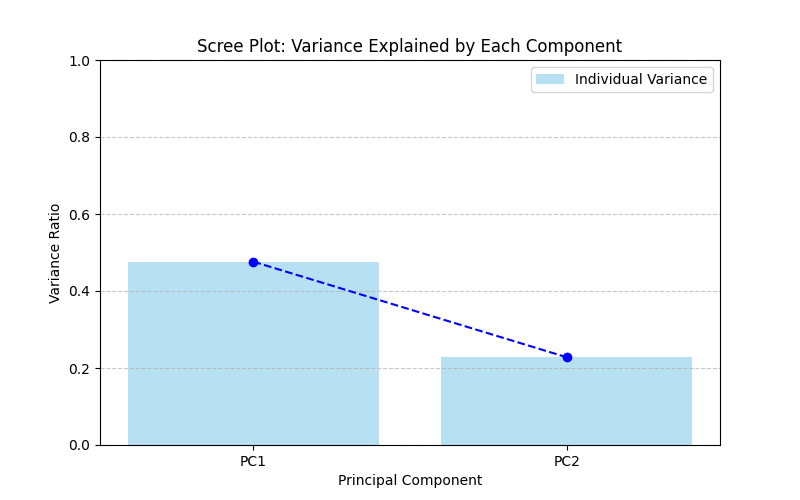
\includegraphics[width=0.7\textwidth]{final_scree_plot.png}
    \caption{Scree Plot showing the variance explained by the first two components.}
    \label{fig:scree}
\end{figure}

\subsection{Model Validation: Reconstruction Error}
To validate the quality of our dimensionality reduction, we calculated the \textbf{Reconstruction Error}. This metric measures the deviation between the original data ($X$) and the data reconstructed from the two principal components ($X_{approx}$). It is defined as the normalized Frobenius norm of the difference:

\begin{equation}
    \text{Error} = \frac{||X - X_{approx}||_F}{||X||_F}
\end{equation}

Our analysis yielded a reconstruction loss of \textbf{0.5439}. This result is mathematically consistent with our Scree Plot analysis. Since our two principal components capture approximately \textbf{70.4\%} of the total variance, the remaining \textbf{29.6\%} accounts for the information loss ($\sqrt{0.296} \approx 0.54$). This confirms that while some fine-grained detail is lost, the 2D projection successfully captures the dominant structural relationships of the disaster dataset.

\newpage
\subsection{Biplot Analysis}
The PCA Biplot (Figure \ref{fig:biplot}) visualizes both the disaster events (points) and the original variables (vectors).

\begin{figure}[h]
    \centering
    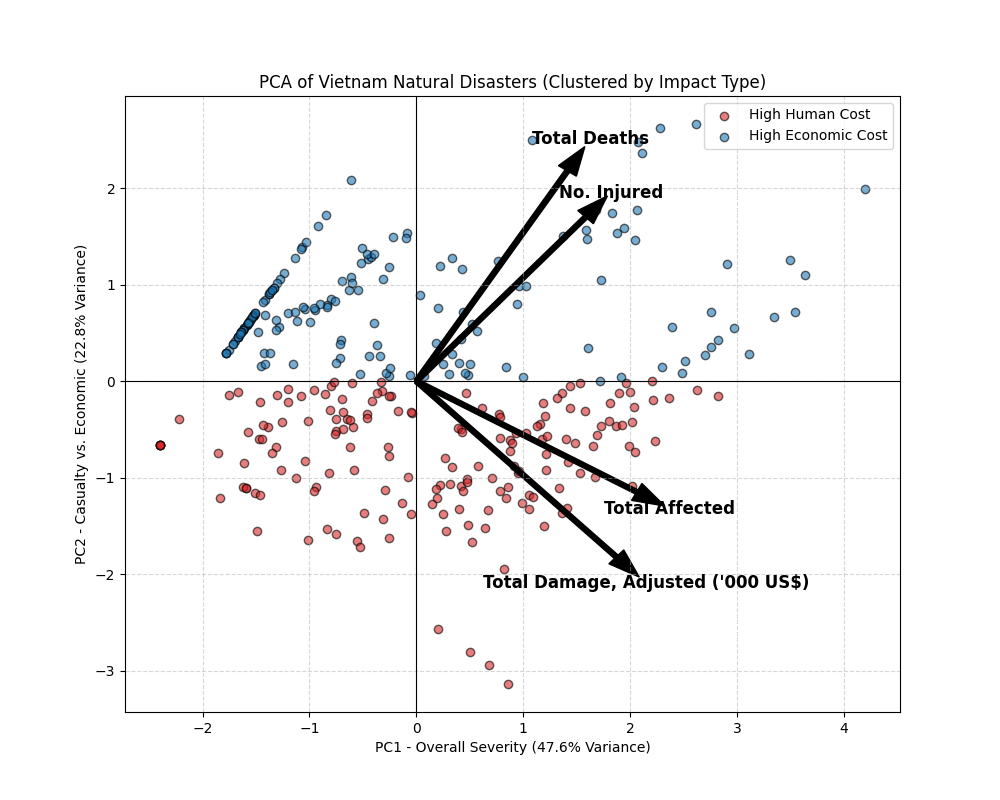
\includegraphics[width=0.8\textwidth]{final_pca_biplot.png}
    \caption{PCA Biplot of Vietnam Natural Disasters (Log-Transformed).}
    \label{fig:biplot}
\end{figure}

\textbf{Interpretation of Axes:}
\begin{itemize}
    \item \textbf{PC1 (Horizontal Axis) - Overall Severity:} All four feature vectors point to the right. This indicates that PC1 represents the general magnitude of a disaster. Events further to the right are historically the most catastrophic in terms of both human and economic cost.
    \item \textbf{PC2 (Vertical Axis) - Human vs. Economic Cost:} This axis reveals a trade-off. "Total Deaths" and "Injured" vectors point downwards, while "Total Damage" points upwards. 
    \begin{itemize}
        \item \textit{Top Quadrant:} Events with high economic damage but fewer casualties (modern storms).
        \item \textit{Bottom Quadrant:} Events with high casualties (deadlier historical events).
    \end{itemize}
\end{itemize}

% --- CONCLUSION ---
\newpage
\chapter{\MakeUppercase{Conclusion}}

In conclusion, PCA is a powerful and practical method for reducing dimensionality, simplifying complex datasets, and revealing their underlying structure. By capturing the directions of greatest variance, it allows us to preserve essential information while removing noise and redundancy.

Whether applied to machine learning, financial analysis, image processing, or biological data, PCA provides a foundation for clearer insights and more efficient models. Understanding how PCA works—and when to use it—helps us analyze data more effectively and make better, data-driven decisions.

% =========================================================
% REFERENCES
% =========================================================
\newpage
\chapter{\MakeUppercase{References}}

\begin{enumerate}
    \item Abdi, H., \& Williams, L. J. (2010). Principal component analysis.
    \textit{WIREs Computational Statistics}, 2(4), 433–459. 
    
    \item Bishop, C. M. (2006).
    \textit{Pattern recognition and machine learning} (Chapter 12). Springer.
    
    \item Duda, R. O., Hart, P. E., \& Stork, D. G. (2012).
    \textit{Pattern classification} (2nd ed., Section 3.8). Wiley.
    
    \item Hastie, T., Tibshirani, R., \& Friedman, J. (2009).
    \textit{The elements of statistical learning: Data mining, inference, and prediction} (2nd ed., Chapter 14.5). Springer.
    
    \item Hotelling, H. (1933).
    Analysis of a complex of statistical variables into principal components. \textit{Journal of Educational Psychology}, 24(6), 417–441.
    
    \item James, G., Witten, D., Hastie, T., \& Tibshirani, R. (2021).
    \textit{An introduction to statistical learning: With applications in R} (2nd ed., Chapter 12). Springer.
    
    \item Jolliffe, I. T. (2002). \textit{Principal component analysis} (2nd ed.). Springer.

    \item Pearson, K. (1901). On lines and planes of closest fit to systems of points in space.
    \textit{Philosophical Magazine}, Series 6, 2(11), 559–572.
    
    \item Shlens, J. (2014).
    A tutorial on principal component analysis. \textit{arXiv preprint arXiv:1404.1100}.
    
    \item Strang, G. (2023).
    \textit{Linear algebra and learning from data} (Chapter 7). Wellesley-Cambridge Press.
    
    \item VanderPlas, J. (2016).
    \textit{Python data science handbook: Essential tools for working with data}. O’Reilly Media.
    
    \item Han, J., Kamber, M., \& Pei, J. (2011).
    \textit{Data Mining: Concepts and Techniques} (3rd ed.). Morgan Kaufmann.
    
    \item Strang, G. (2016). \textit{Introduction to Linear Algebra} (5th ed.).
    Wellesley-Cambridge Press.

    % --- NEW REFERENCES ADDED FROM FILE ---
    \item Shlens, J. (2005). ``Notes on principal component analysis,'' Google Research.
    [Online]. Available: \url{https://www.cs.princeton.edu/picasso/mats/PCA-Tutorial-Intuition_josh.pdf}
    
    \item ``Principal Component Analysis (PCA) explained,'' Towards Data Science.
    [Online]. Available: \url{https://towardsdatascience.com/pca-explained}
\end{enumerate}

\end{document}